% Chapter Template

\Appendix{Examples} % Main chapter title

\label{sec:Examples} % Change X to a consecutive number; for referencing this chapter elsewhere, use \ref{ChapterX}


In this appendix, I will go through many examples, illustrating how to use the code base to create, learn and solve various puzzles. For each section, a snippet of code will be indicated in \afblue \textbf{python code} \black paragraphs, and can easily be run from command line or copied into a script and run from your favourite Python IDE.


%-----------------------------------
%	SECTION 1
%-----------------------------------
\Section{Puzzles}
Let me start by showing how to construct puzzles, using the Puzzle factory. Notice that in order to run a learner or solver of any kind (assuming of course that they are meant to work on the puzzle type in question), we can just use the exact same code, simply specifying \textit{puzzle\_type} and the expected parameters to construct a puzzle. The factories will just pick up the relevant parameters indicating the puzzle type and dimension and everything should work seamlessly.
\\
\\
For instance, let us create a 5x6 \textbf{SP}, shuffle it a thousand times, and print it:
\afblue
\paragraph{}{\textbf{python code -- sliding puzzle construction}}
\begin{python}
####################################################################
from rubiks.puzzle.puzzle import Puzzle
####################################################################
puzzle_type=Puzzle.sliding_puzzle
n=5
m=6
nb_moves=1000
print(Puzzle.factory(**globals()).apply_random_moves(nb_moves))
####################################################################
\end{python}
\black
The output from the above code snippet will look like (subject to randomness):

\begin{figure}[H]
\centering
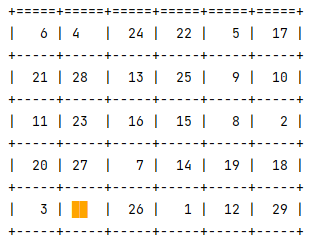
\includegraphics[scale=0.8]{./Figures/examplespconstruction}
%\decoRule
\caption[Examples]{scrambled 5x6 \textbf{SP} example}
\label{fig:examplespconstruction}
\end{figure}
.. similarly to construct a perfectly scrambled 2x2x2 \textbf{RC}:
\afblue
\paragraph{}{\textbf{python code -- Rubik's cube construction}}
\begin{python}
####################################################################
from math import inf
from rubiks.puzzle.puzzle import Puzzle
####################################################################
puzzle_type=Puzzle.rubiks_cube
n=2
""" Here we use perfect shuffle by spcifying infinite number of shuffles """
nb_moves=inf
print(Puzzle.factory(**globals()).apply_random_moves(nb_moves))
####################################################################
\end{python}
\black

\begin{figure}[H]
\centering
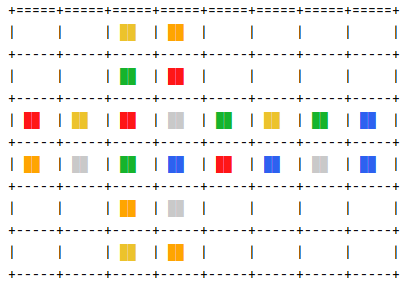
\includegraphics[scale=0.8]{./Figures/examplercconstruction}
%\decoRule
\caption[Examples]{rubiks cube construction example}
\label{fig:examplercconstruction}
\end{figure}


%-----------------------------------
%	SECTION 2
%-----------------------------------
\Section{Learners}


%-----------------------------------
%	SUBSECTION 2.1
%-----------------------------------
\Subsection{Perfect Learner}
\label{PLSS}

The perfect learner has been discussed in details in \ref{sec:codelearners}. We simply show here how to run it to learn the value function for the 2x3 \textbf{SP}, that is, to solve all 360 possible configurations via an optimal solver (A{*} with Manhattan heuristic).


\afblue
\paragraph{}{\textbf{python code -- perfect learner}}
\begin{python}
####################################################################
from rubiks.heuristics.heuristic import Heuristic
from rubiks.puzzle.puzzle import Puzzle
from rubiks.learners.learner import Learner
from rubiks.utils.utils import get_model_file_name
####################################################################
action_type=Learner.do_learn
n=2
m=3
puzzle_type=Puzzle.sliding_puzzle
learner_type=Learner.perfect_learner
heuristic_type=Heuristic.manhattan
nb_cpus=4
learning_file_name=get_model_file_name(puzzle_type=puzzle_type,
                                       dimension=(n, m),
                                       model_name=Learner.perfect)
if __name__ == '__main__':
    # we fully solve the 2 x 3 SP ... should take ~5s
    Learner.factory(**globals()).action()
####################################################################
action_type=Learner.do_plot
if __name__ == '__main__':
    # we display the results
    Learner.factory(**globals()).action()
####################################################################
\end{python}
\black
The above snippet of code solves the 2x3 \textbf{SP} and then displays the results, showing the distribution of optimal costs, as well as the most difficult puzzle:

\begin{figure}[H]
\centering
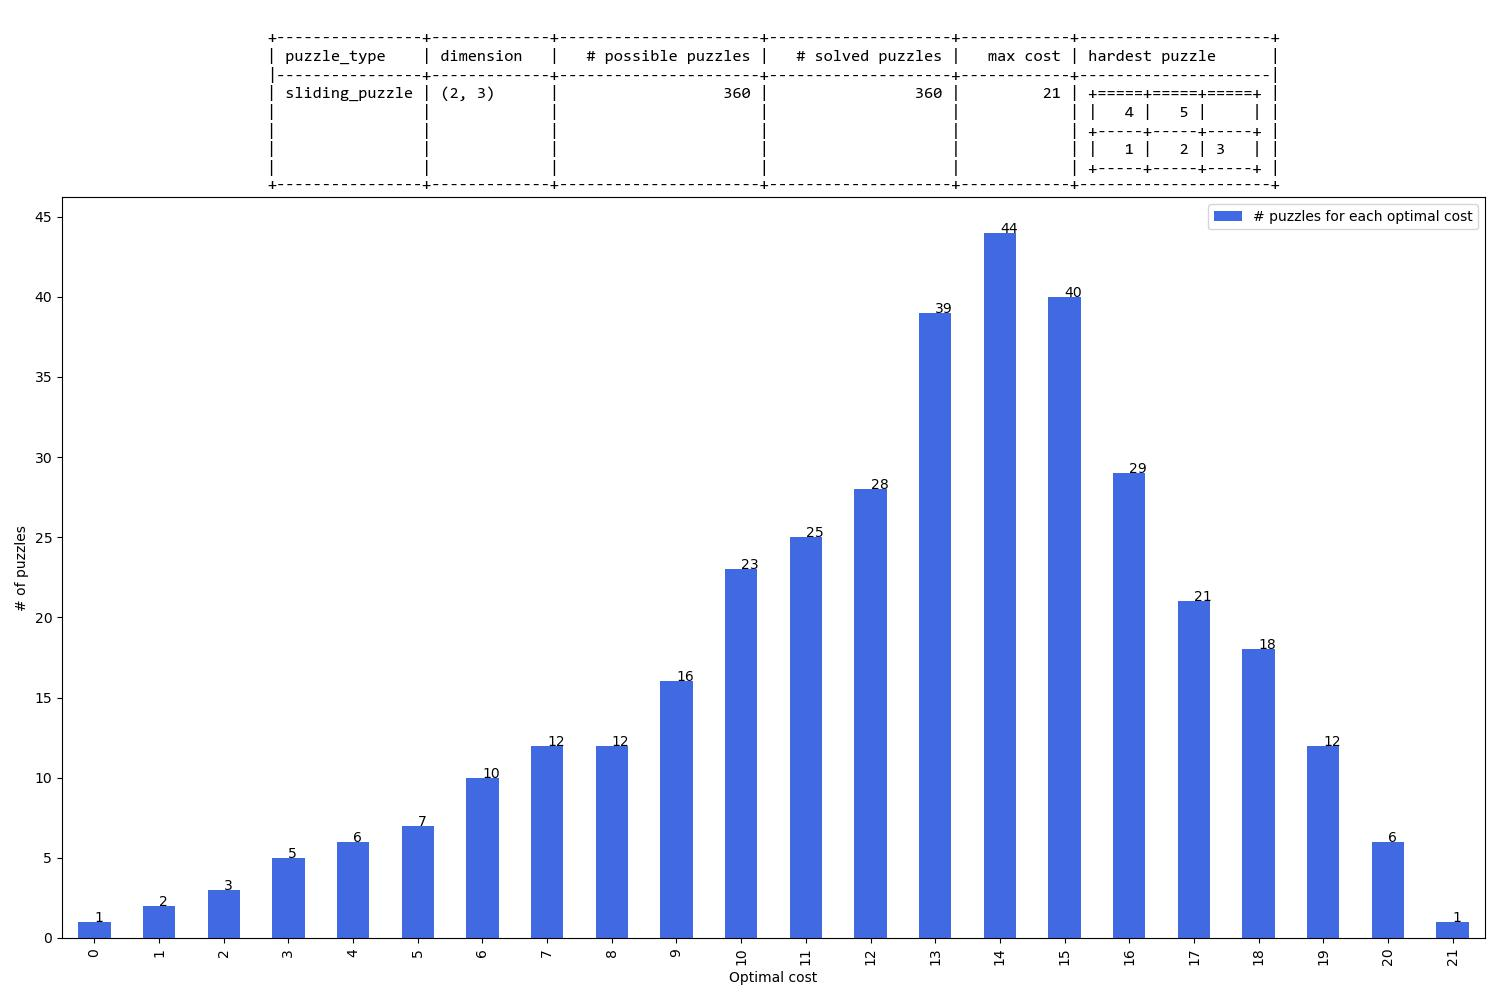
\includegraphics[scale=0.41]{./Figures/exampleperfectlearner}
%\decoRule
\caption[Examples]{perfect learner example}
\label{fig:exampleperfectlearner}
\end{figure}


%-----------------------------------
%	SUBSECTION 2.2
%-----------------------------------
\Subsection{Deep Learner}
\label{DLSS}
The DeepLearner, also discussed in details in \ref{sec:codelearners}, needs some training data. It could in principle of course be trained on any data, not necessarily optimal data (i.e. generated by an optimal solver). Here however, I make use of the TrainingData class to generate 100 sequences of fully solved 5x2 \textbf{SP} via A{*} with Manhattan++.


\afblue
\paragraph{}{\textbf{python code -- deep learner}}
\begin{python}
####################################################################
from math import inf
####################################################################
from rubiks.deeplearning.deeplearning import DeepLearning
from rubiks.learners.learner import Learner
from rubiks.learners.deeplearner import DeepLearner
from rubiks.puzzle.puzzle import Puzzle
from rubiks.puzzle.trainingdata import TrainingData
####################################################################
if '__main__' == __name__:
    puzzle_type=Puzzle.sliding_puzzle
    n=5
    m=2
    """ Generate training data - 100 sequences of fully 
    solved perfectly shuffled puzzles. 
    """
    nb_cpus=4
    time_out=600
    nb_shuffles=inf
    nb_sequences=100
    TrainingData(**globals()).generate(**globals())
    """ DL learner """
    action_type=Learner.do_learn
    learner_type=Learner.deep_learner
    nb_epochs=999
    learning_rate=1e-3
    optimiser=DeepLearner.rms_prop
    scheduler=DeepLearner.exponential_scheduler
    gamma_scheduler=0.9999
    save_at_each_epoch=False
    threshold=0.01
    training_data_freq=100
    high_target=nb_shuffles + 1
    training_data_from_data_base=True
    nb_shuffles_min=20
    nb_shuffles_max=50
    nb_sequences=50
    """ ... and its network config """
    network_type=DeepLearning.fully_connected_net
    layers_description=(100, 50, 10)
    one_hot_encoding=True
    """ Kick-off the Deep Learner """
    learning_file_name=Learner.factory(**globals()).get_model_name()
    Learner.factory(**globals()).action()
    """ Plot its learning """
    action_type=Learner.do_plot
    Learner.factory(**globals()).action()
####################################################################
\end{python}
\black

As can be seen in the code snippet, this example will generate 100 perfectly shuffled (n=5, m=2) SPs and solve them. Once done, a summary of the training data is printed, indicating, for each optimal cost, how many sequences have been generated.

\begin{figure}[H]
\centering
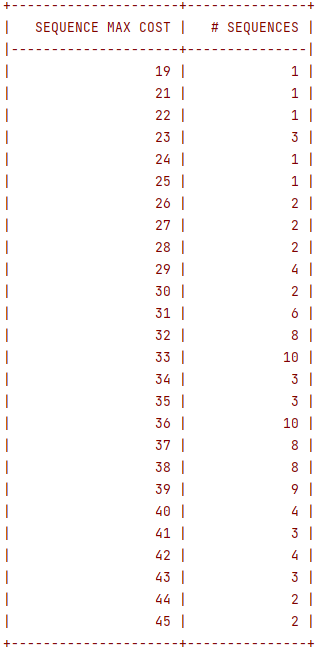
\includegraphics[scale=0.45]{./Figures/exampledeeplearnertraining}
%\decoRule
\caption[Examples]{deep learner training example}
\label{fig:exampledeeplearnertraining}
\end{figure}

Then the Deep Learner will get trained on this data for 999 epochs. In the above example, I have chosen to fetch, every 100 epochs, 50 random sequences of puzzles from the training data. Each sequence is composed of a random puzzle of cost between 20 and 50, fetched from the training data, along with its optimal path to the solution. The default optimiser (rms\_prop) is used, together with an exponential scheduler starting with a learning rate of 0.001 and a gamma of 0.9999. We can see that the (MSE) loss on the value function decreases rapidly, and jumps back up every time we change the training data (since it has not yet seen some of it). By the end of the training, the in-sample MSE loss has dropped to 1.5 and the Deep Learner has seen 0.14\% of the possible (n=5, m=2) puzzles.

\newgeometry{top=0mm, bottom=0mm, left=0mm, right=0mm}
\begin{landscape}
\centering\vspace*{\fill}
\begin{figure}[H]
\centering
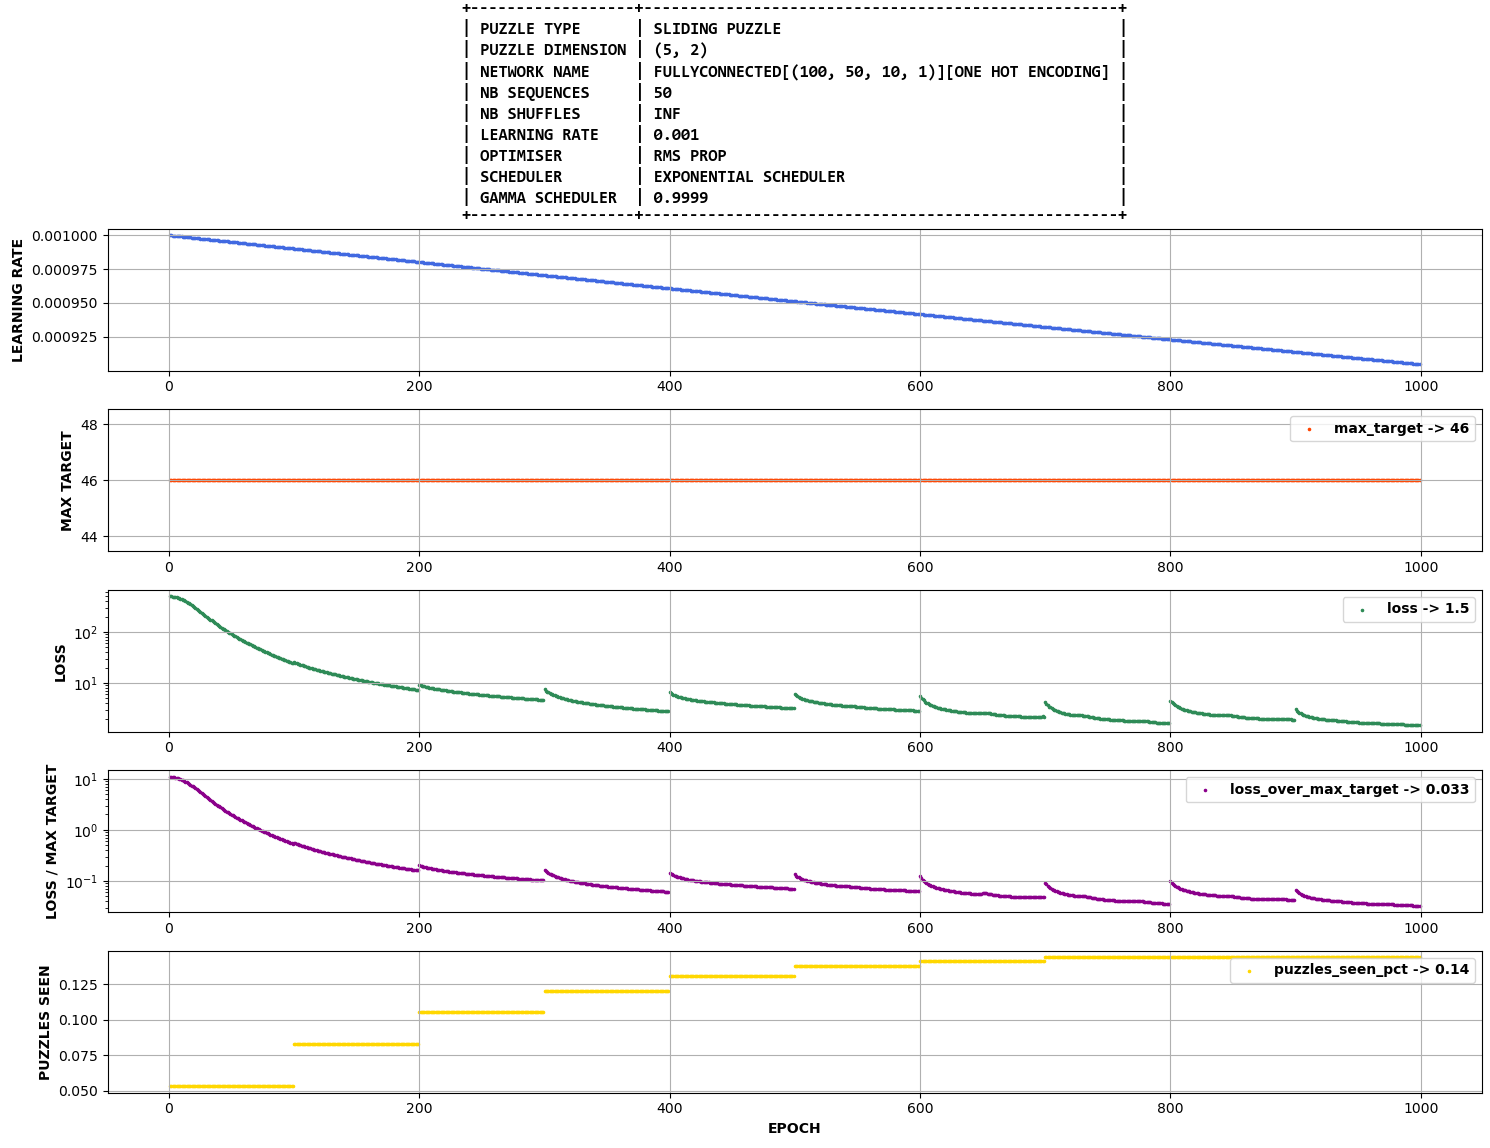
\includegraphics[scale=0.45]{./Figures/exampledeeplearnerlearning}
%\decoRule
\caption[Examples]{deep learner learning data example}
\label{fig:exampledeeplearnerlearning}
\end{figure}
\vfill
\end{landscape}
\restoregeometry






%-----------------------------------
%	SUBSECTION 2.3
%-----------------------------------
\Subsection{Deep Reinforcement Learner}
\label{DRLSS}

Unlike the Deep Learner, the Deep Reinforcement Learner learns unsupervised (in the sense that there is no need to pre-solve puzzles to tell if what the actual (target) costs are), since it generates its own target using a combination of a target network and the simple min rule described in \ref{sec:codelearners}. Let us see here how to run it on the (n=4, m=2) SP for instance. The following code snippet will run a Deep Reinforcement Learner for a maximum of 25,000 epochs, generating randomly 10 sequences of puzzles shuffled 50 times from goal state every time it updates the target network. That update will happen either after 500 epochs or when the (MSE) loss on the value function gets under one thousands of the max target value. The learner will stop if it reaches 25,000 epochs or if the target network updates 40 times. The network trained is a fully connected network with 3 hidden layers and the puzzles are one-hot encoded. We use the same optimiser and scheduler as in the previous subsection.

\afblue
\paragraph{}{\textbf{python code -- deep reinforcement learner}}
\begin{python}
####################################################################
from rubiks.deeplearning.deeplearning import DeepLearning
from rubiks.learners.learner import Learner
from rubiks.learners.deepreinforcementlearner import DeepReinforcementLearner
from rubiks.puzzle.puzzle import Puzzle
####################################################################
if '__main__' == __name__:
    puzzle_type=Puzzle.sliding_puzzle
    n=4
    m=2
    """ Generate training data - 100 sequences of fully 
    solved perfectly shuffled puzzles. 
    """
    nb_cpus=4
    """ DRL learner """
    action_type=Learner.do_learn
    learner_type=Learner.deep_reinforcement_learner
    nb_epochs=25000
    nb_shuffles=50
    nb_sequences=10
    training_data_every_epoch=False
    cap_target_at_network_count=True
    update_target_network_frequency=500
    update_target_network_threshold=1e-3
    max_nb_target_network_update=40
    max_target_not_increasing_epochs_pct=0.5
    max_target_uptick=0.01
    learning_rate=1e-3
    scheduler=DeepReinforcementLearner.exponential_scheduler
    gamma_scheduler=0.9999
    """ ... and its network config """
    network_type=DeepLearning.fully_connected_net
    layers_description=(128, 64, 32)
    one_hot_encoding=True
    """ Kick-off the Deep Reinforcement Learner ... """
    learning_file_name=Learner.factory(**globals()).get_model_name()
    Learner.factory(**globals()).action()
    """ ... and plot its learning data """
    action_type=Learner.do_plot
    Learner.factory(**globals()).action()
####################################################################
\end{python}
\black
As can be seen on the next page, which I obtained from running the above code snippet (keep in mind that every run is going to be slightly different due to the random puzzles being generated), the training stopped after about 17,100 epochs as the 40 target network updates had been reached. By that point, the DRL learner had seen 40\% of the possible puzzles, and the very last MSE loss (after update, so out-of-sample) was around 0.4, corresponding to 2\% of the max target cost. It is interesting to notice that since I have shuffled the sequences only 50 times, and since the (n=4, m=2) SP is quite constrained in terms of possible moves, the max target ever produced by the network was only around 25, whereas we know the God number for this dimension is 36 (see later section \ref{sec:SPLowDimension}). It is therefore likely that the resulting network would not produce very optimal solutions for puzzles whose cost is in the region [25, 36]. 


\newgeometry{top=0mm, bottom=0mm, left=0mm, right=0mm}
\begin{landscape}
\centering\vspace*{\fill}
\begin{figure}[H]
\centering
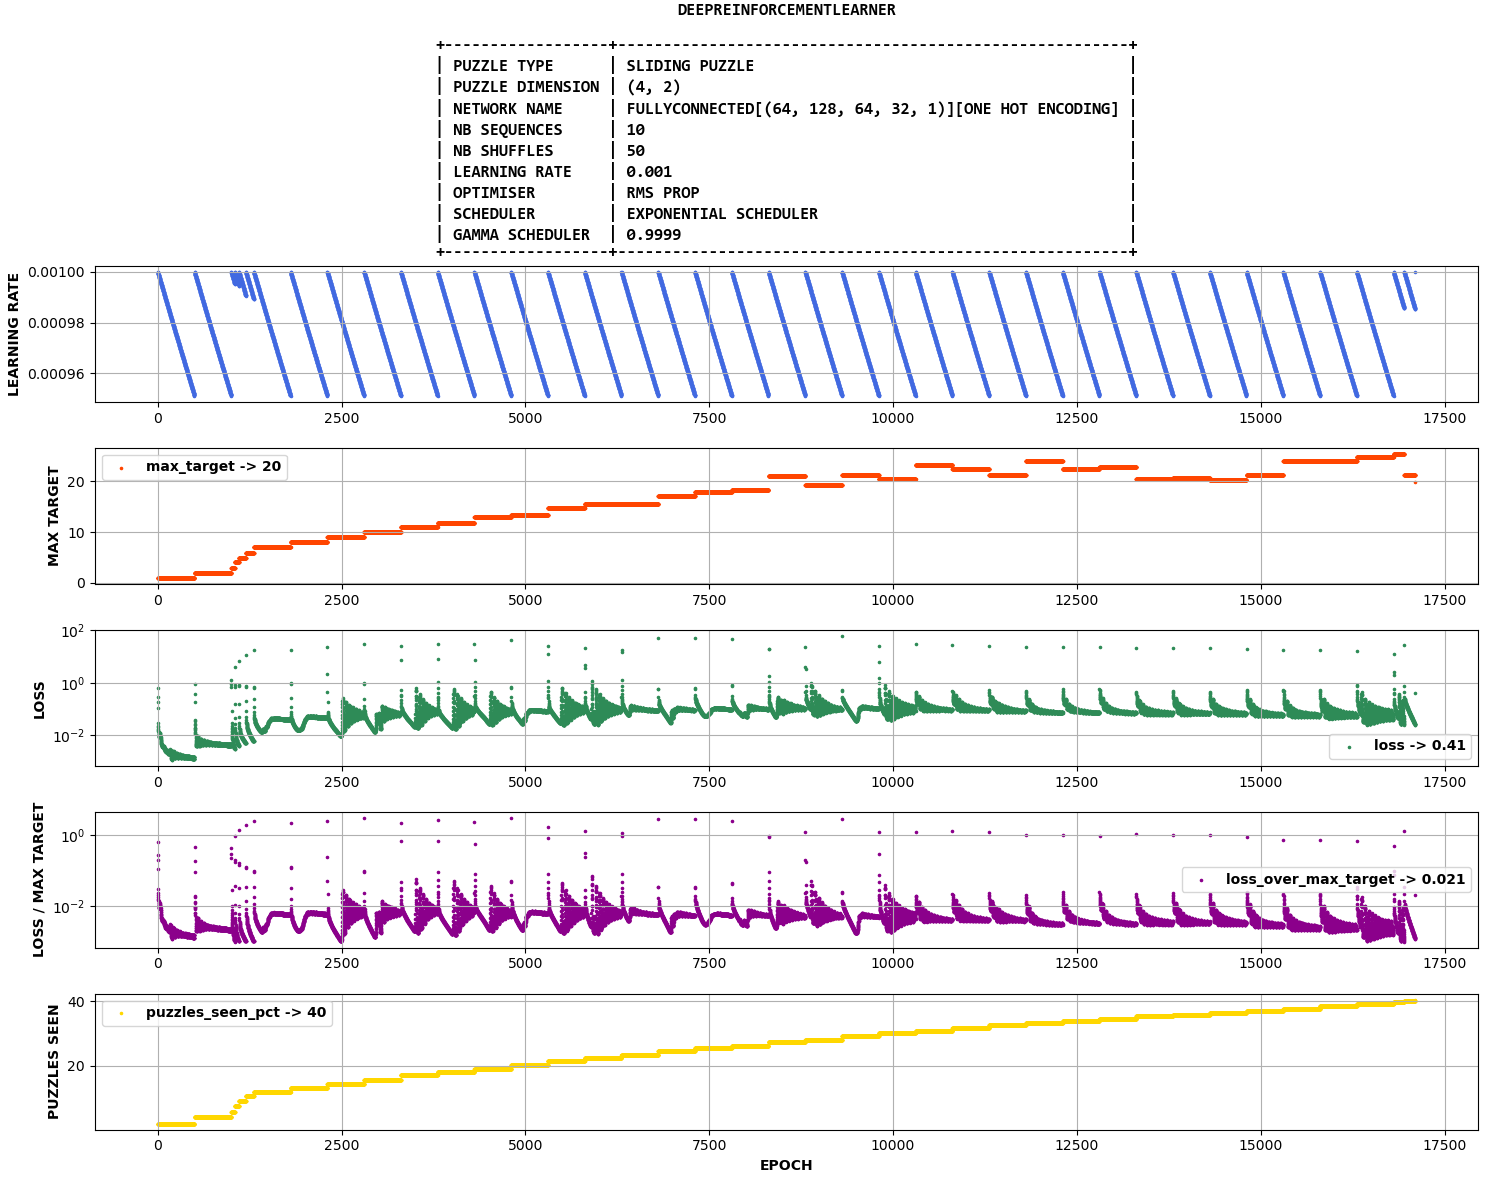
\includegraphics[scale=0.55]{./Figures/exampledeepreinforcementlearnerlearning}
%\decoRule
\caption[Examples]{deep reinforcement learner learning data example}
\label{fig:exampledeepreinforcementlearnerlearning}
\end{figure}
\vfill
\end{landscape}
\restoregeometry





%-----------------------------------
%	SECTION 3
%-----------------------------------

\Section{Solvers}

%-----------------------------------
%	SUBSECTION 3.1
%-----------------------------------
\Subsection{Blind search}
First let me start with some of the blind search algorithms, which I only have been able to use on small dimension SP. They quickly become too memory hungry to be practical on anything but the smallest puzzles.
%-----------------------------------
%	SUBSECTION 3.1.1
%-----------------------------------
\Subsubsection{BFS}
\label{BFSSS}
The following example shows how to use Breadth First Search to solve a (n=3, m=3) SP which we do not \textit{shuffle} too much.

\afblue
\paragraph{}{\textbf{python code -- breadth first search solver}}
\begin{python}
####################################################################
from rubiks.solvers.solver import Solver
from rubiks.puzzle.puzzle import Puzzle
####################################################################
if '__main__' == __name__:
    puzzle_type = Puzzle.sliding_puzzle
    n=3
    m=3
    nb_shuffles=10
    solver_type=Solver.bfs
    check_optimal=True
    action_type=Solver.do_solve
    print(Solver.factory(**globals()).action())
####################################################################
\end{python}
\black

As expected (since BFS is optimal), the solution found, printed by the snippet of code above, is optimal. The check\_optimal flag in the code snippet indicates that the solver should let us know if solution is optimal. Since BFS advertises itself (via the Solver base class API)  as an optimal solver, the solution is deemed optimal.


\begin{figure}[H]
\centering
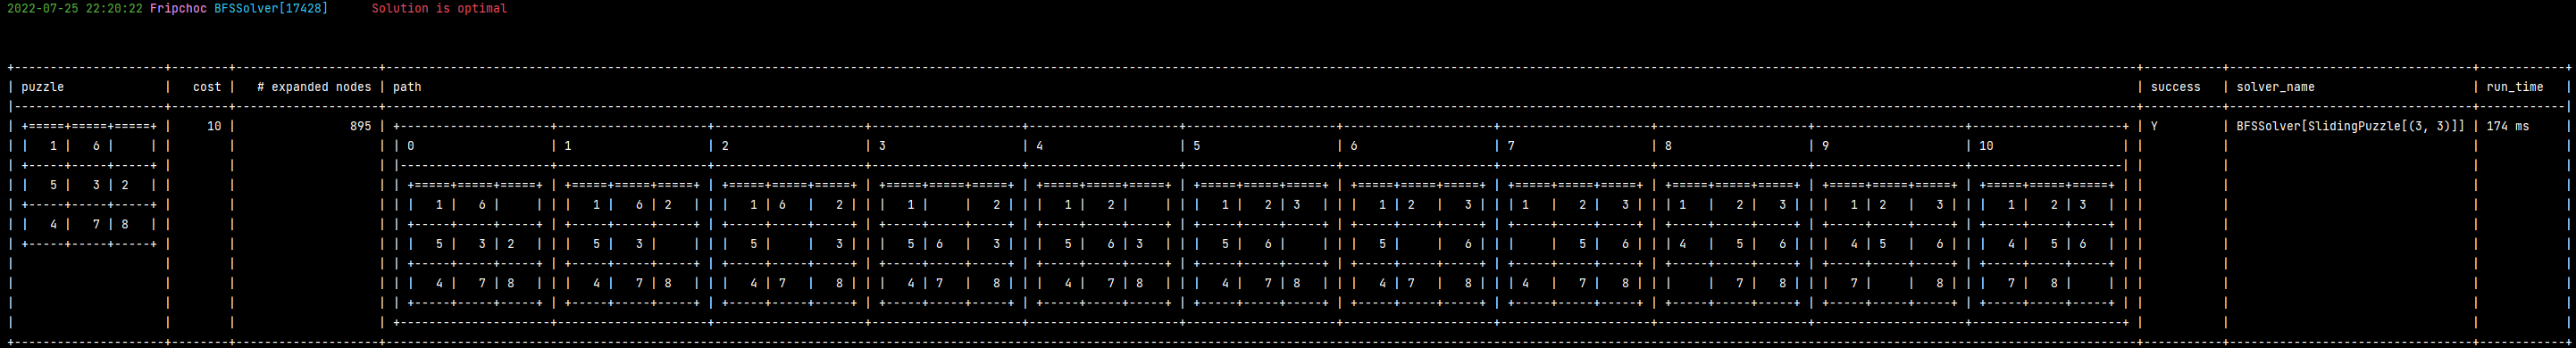
\includegraphics[scale=0.25]{./Figures/examplebfssolver}
%\decoRule
\caption[Examples]{breadth first search solver example}
\label{fig:examplebfssolver}
\end{figure}

%-----------------------------------
%	SUBSECTION 3.1.2
%-----------------------------------
\Subsubsection{DFS}
\label{DFSSS}



\afblue
\paragraph{}{\textbf{python code -- depth first search solver}}
\begin{python}
####################################################################
from rubiks.solvers.solver import Solver
from rubiks.puzzle.puzzle import Puzzle
####################################################################
if '__main__' == __name__:
    puzzle_type = Puzzle.sliding_puzzle
    n=3
    m=3
    nb_shuffles=8
    limit=15
    time_out=60
    solver_type=Solver.dfs
    check_optimal=True
    log_solution=True
    action_type=Solver.do_solve
    Solver.factory(**globals()).action()
####################################################################

\end{python}
\black
Here we can see, in contrast with the previous example, that the solution obtained by DFS is not optimal. The Solver indicates it and shows an optimal solution. Clearly since we shuffled 8 times from goal configuration, the optimal path cannot have a cost higher than 8 (it could be lower though of course).

\begin{figure}[H]
\centering
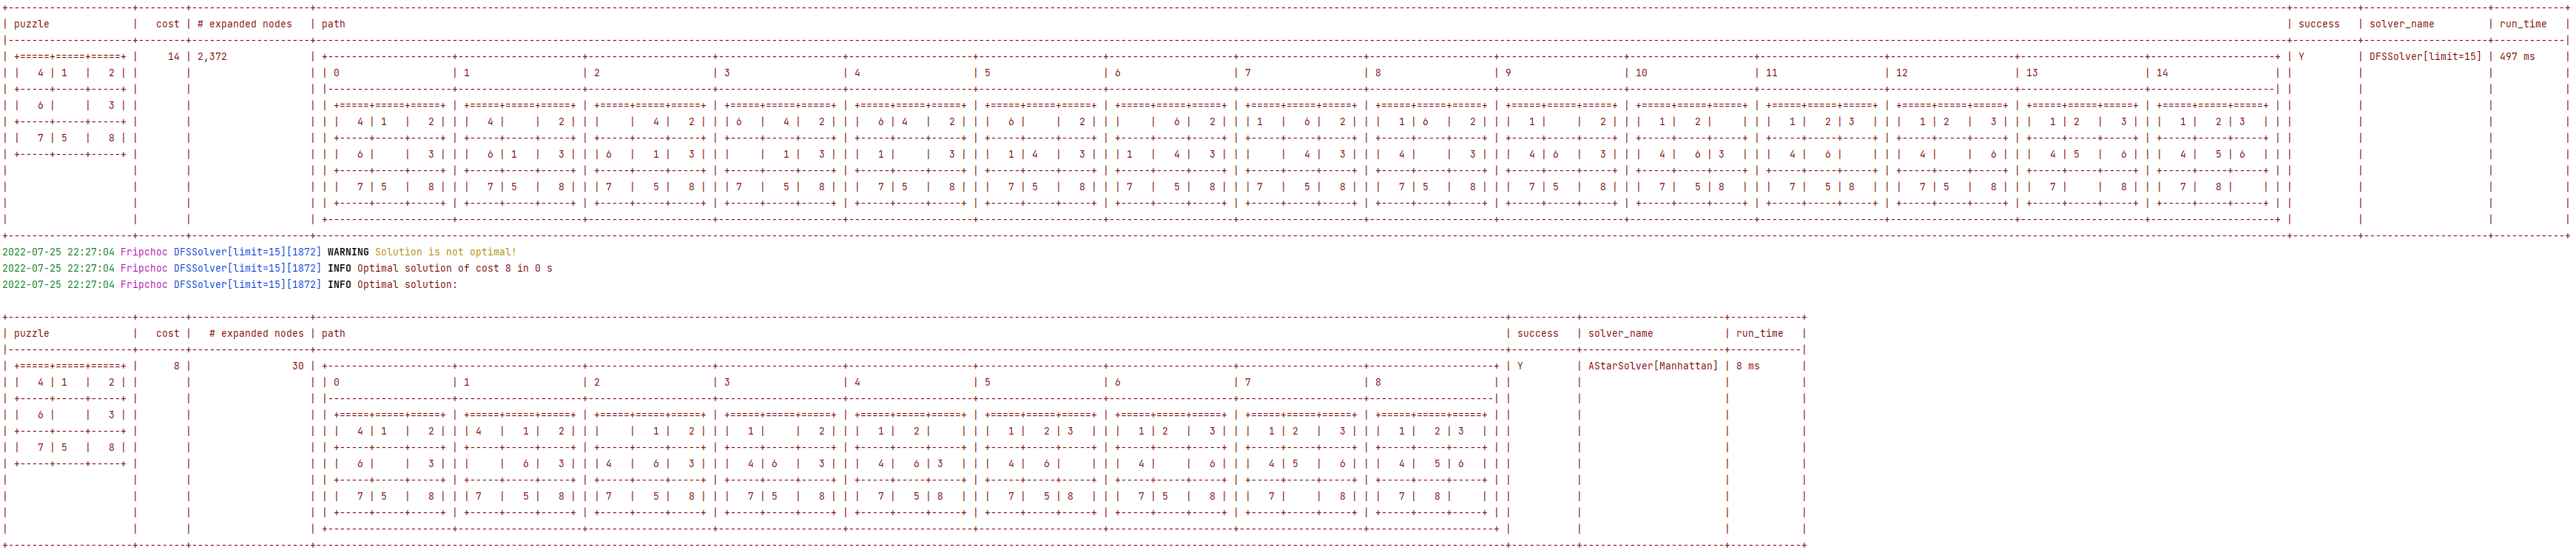
\includegraphics[scale=0.2]{./Figures/exampledfssolver}
%\decoRule
\caption[Examples]{depth first search solver example}
\label{fig:exampledfssolver}
\end{figure}


%-----------------------------------
%	SUBSECTION 3.2
%-----------------------------------
\Subsection{Naive Sliding Puzzle Solver}
As a comparison point for otherSP solvers, I have implemented a naive sliding puzzle solver, which does what most beginner players would intuitively do when solving the sliding puzzle by hand: solve the top row, then the left column, and keep iterating until done. Notice that once either the top row or left column is solved, there is no longer any need to modify it, we have simply reduced the problem to a sub-problem of reduced dimension. For the interested reader, the details of the algorithm are as follows:
\begin{itemize}
\item if n and m are both equal to 2, we just keep moving the empty tile clock-wise until the puzzle is solved. Notice that this is bound to work, since moving clock-wise or counter-clock-wise are the two ony possible moves, and one of them is just un-doing the other one, therefore the only possible sequence of move in a (n=2, m=2) puzzle is to either keep moving clock-wise or counter-clock-wise.
\item if n $\geq$ m, we solve the top row
\item otherwise we solve the left column
\end{itemize}
Solving the top row of a n by m puzzle (left column is similar, mutatis mutandis, so I will not detail it) is accomplished as follows:
\\
\textbf{naive algorithm - top-row solver}
\begin{enumerate}
\item \label{s1} we sort the tiles (which since we are potentially dealing with a sub-problem, are not necessarily 1 to $m* n - 1$), and select the m smaller ones $t_{1}, ..., t_{m-1}, t_{m}$.
\item \label{s2} we place $t_{m}$ in the bottom-left corner
\item \label{s3} we place $t_{1}, ..., t_{m-2}$ to their respective positions (in that order, and making sure not to undo any previous steps as we do so)
\item \label{s4} we place $t_{m-1}$ in the top-right corner
\item \label{s5} we then move $t_{m}$ just under $t_{m-1}$
\item \label{s6} we move the empty tile to the left of $t_{m-1}$
\item \label{s7} finally we move the empty tile right and then down to put $t_{m-1}$ and $t_{m}$ in place.
\end{enumerate}
In order to move the tiles, we have written a few simple routines which can move the empty tile from its current position next to (above, below, left or right) any tile, and then can move that tile to another position, all the while avoiding to go through previously moved tiles (hence the particular order in which we move the different tiles above). The only case where the above algorithm can get stuck is when both n and m are equal to 3 and that by step \ref{s6} we end up with $t_{3}$ under the empty tile. We have handcrafted a sequence of moves to solve this particular position. Other than this one particular case, the above naive algorithm is guaranteed to succeed (and is obviously quite fast in terms of run time, though not elegant).
\\
\\
As a concrete example, let us assume we started with the following (n=6, m=6) puzzle:
\\
\begin{thityfive}
\setrow{6}{14,27,6,  2,5,18}
\setrow{5}{21,29,13,23,35,30}
\setrow{4}{26,3,7,9,24,19}
\setrow{3}{22,12,11,17,16,33}
\setrow{2}{32,10,20,25,34,28}
\setrow{1}{8,4,15,31, ,1}
\end{thityfive}
\\
\\
After one call to solve the top row and the left column, we are left with solving the (n=5,m=5) sub-puzzle in blue:
\\
\begin{thityfive}
\setrow{6}{1,2,3,4,5,6}
\setrow{5}{7,\blue9,\blue17,\blue27,\blue18,\blue35}
\setrow{4}{8,\blue23,\blue11,\blue15,\blue24,\blue21}
\setrow{3}{9,\blue20,\blue8,\blue29,\blue33,\blue10}
\setrow{2}{10,\blue22,\blue30,\blue14,\blue32,\blue16}
\setrow{1}{11,\blue ,\blue12,\blue26,\blue34,\blue28}
\end{thityfive}
\\
\\
Let us now detail how the \textbf{naive algorithm} will solve the top row if that sub-puzzle:
\\
\begin{twentyfour}
\setrow{5}{9,17,27,18,35}
\setrow{4}{23,11,15,24,21}
\setrow{3}{20,8,29,33,10}
\setrow{2}{22,30,14,32,16}
\setrow{1}{ ,12,26,34,28}
\end{twentyfour}
\\
\\
step \ref{s1} above will decide to solve the top row by placing $t_{1}, ..., t_{5}$ = $\blue 8, 9, 10, 11, 12$ in that order as the top row. Steps \ref{s2} to \ref{s7} will yield in order:
\\
\begin{twentyfour}
\setrow{5}{\blue9,17,27,18,35}
\setrow{4}{23,\blue11,15,24,21}
\setrow{3}{20,\blue8,29,33,\blue10}
\setrow{2}{22,30,14,32,16}
\setrow{1}{ ,\blue12,26,34,28}
\end{twentyfour}
%
\begin{twentyfour}
\setrow{5}{\blue9,17,27,18,35}
\setrow{4}{23,\blue11,15,24,21}
\setrow{3}{20,\blue8,29,33,\blue10}
\setrow{2}{22,30,14,32,16}
\setrow{1}{\color{red}12\color{red}, ,26,34,28}
\end{twentyfour}
%
\begin{twentyfour}
\setrow{5}{\red 8,\red 9,\red 10,,18}
\setrow{4}{17,15,27,24,35}
\setrow{3}{\blue11,23,29,21,33}
\setrow{2}{20,22,14,32,16}
\setrow{1}{\red 12,30,26,34,28}
\end{twentyfour}
\\
\begin{twentyfour}
\setrow{5}{\red 8, \red 9, \red 10,,\red 11}
\setrow{4}{23,29,21,18,24}
\setrow{3}{17,15,27,33,35}
\setrow{2}{20,22,14,32,16}
\setrow{1}{\red 12,30,26,34,28}
\end{twentyfour}
%
\begin{twentyfour}
\setrow{5}{\red 8,\red 9,\red 10,18,\red 11}
\setrow{4}{29,27,32, ,\red 12}
\setrow{3}{23,21,33,35,24}
\setrow{2}{15,17,22,14,16}
\setrow{1}{30,20,26,34,28}
\end{twentyfour}
%
\begin{twentyfour}
\setrow{5}{\red 8, \red 9, \red 10, \red 11, \red 12}
\setrow{4}{29,27,32,18, }
\setrow{3}{23,21,33,35,24}
\setrow{2}{15,17,22,14,16}
\setrow{1}{30,20,26,34,28}
\end{twentyfour}
\\
\\
and we are left with solving the bottom sub-puzzle (n=4,m=5):
\\
\begin{twenty}
\setrow{4}{29,27,32,18, }
\setrow{3}{23,21,33,35,24}
\setrow{2}{15,17,22,14,16}
\setrow{1}{30,20,26,34,28}
\end{twenty}
\\
\\
which the naive solver can keep solving iteratively by taking care of the left-most column, etc...
\\
\\
Below is a simple code snippet to run the naive solver on a randomly generated (n=2, m=2) SP:
\afblue
\paragraph{}{\textbf{python code -- naive solver}}
\begin{python}
################################################
from math import inf
from rubiks.puzzle.puzzle import Puzzle
from rubiks.solvers.solver import Solver
################################################
action_type=Solver.do_solve
n=2
puzzle_type=Puzzle.sliding_puzzle
solver_type=Solver.naive
nb_shuffles=inf
################################################
print(Solver.factory(**globals()).action())
################################################
\end{python}
\black

\begin{figure}[H]
\centering
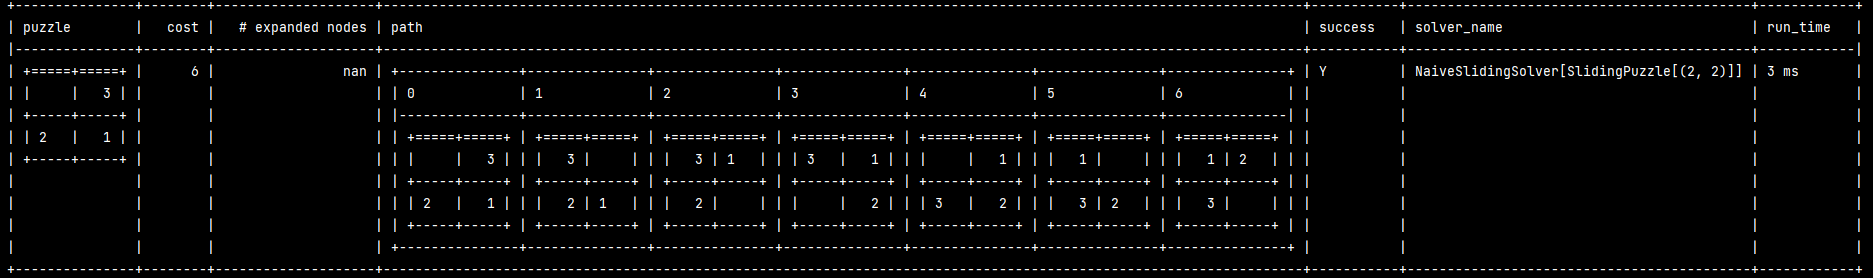
\includegraphics[scale=0.39]{./Figures/examplenaivesolver}
%\decoRule
\caption[Examples]{naive solver example}
\label{fig:examplenaivesolver}
\end{figure}



%-----------------------------------
%	SUBSECTION 3.3
%-----------------------------------
\Subsection{Kociemba}


\afblue
\paragraph{}{\textbf{python code -- Kociemba solver}}
\begin{python}
####################################################################
from rubiks.puzzle.puzzle import Puzzle
from rubiks.solvers.solver import Solver
####################################################################
puzzle_type=Puzzle.rubiks_cube
n=2
cube=Puzzle.factory(**globals()).apply_random_moves(2)
solver_type=Solver.kociemba
solver = Solver.factory(**globals())
print(solver.solve(cube))
####################################################################

\end{python}
\black

\begin{figure}[H]
\centering
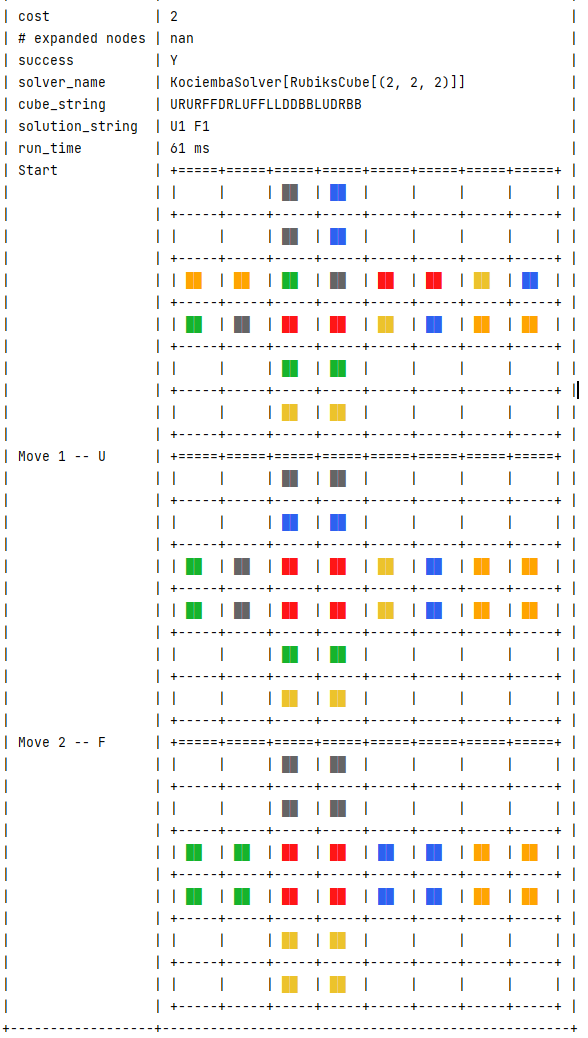
\includegraphics[scale=0.55]{./Figures/examplekociemba}
%\decoRule
\caption[Examples]{Kociemba solver example}
\label{fig:examplekociemba}
\end{figure}



%-----------------------------------
%	SUBSECTION 3.4
%-----------------------------------
\Subsection{A*}
\label{ASSS}

\Subsubsection{Manhattan heuristic}



\afblue
\paragraph{}{\textbf{python code -- depth first search solver}}
\begin{python}
####################################################################
from rubiks.heuristics.heuristic import Heuristic
from rubiks.puzzle.puzzle import Puzzle
from rubiks.solvers.solver import Solver
####################################################################
if '__main__' == __name__:
    puzzle_type = Puzzle.sliding_puzzle
    tiles=[[3, 8, 6], [4, 1, 5], [0, 7, 2]]
    solver_type=Solver.astar
    heuristic_type=Heuristic.manhattan
    plus=False
    action_type=Solver.do_solve
    print(Solver.factory(**globals()).action().to_str_light())
####################################################################
\end{python}
\black
We run this example twice, one with simple Manhattan and one with Manhattan++. As can be seen from the output below, the Manhattan++ improves on the number of expanded nodes (as expected, since the heuristic is less optimistic while retaining its optimality property). See a more detailed analysis in the SP results section \ref{}

\begin{figure}[H]
\centering
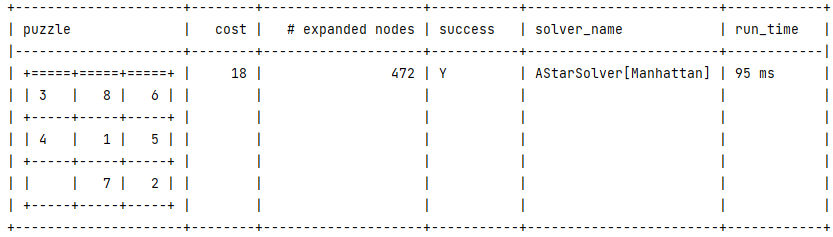
\includegraphics[scale=0.5]{./Figures/exampleastarmanhattansolver}
%\decoRule
\caption[Examples]{a* manhattan solver example}
\label{fig:exampleastarmanhattansolver}
\end{figure}

\begin{figure}[H]
\centering
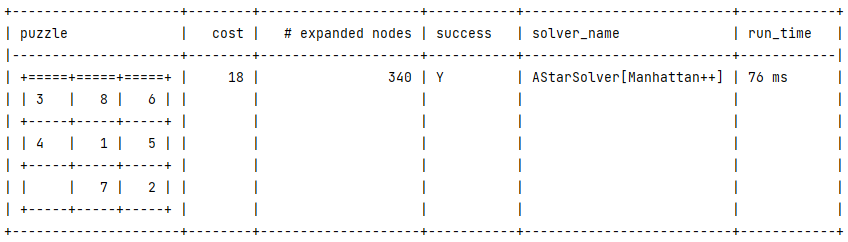
\includegraphics[scale=0.5]{./Figures/exampleastarmanhattanplussolver}
%\decoRule
\caption[Examples]{a* manhattan++ solver example}
\label{fig:exampleastarmanhattanplussolver}
\end{figure}



\Subsubsection{Perfect Heuristic}
To run A{*} with a perfect heuristic, we just need to specify the heuristic type as such, and set the parameter \textit{model\_file\_name} to point to a pre-recorded database populated by the PerfectLearner (see earlier section \ref{PLSS}).


\afblue
\paragraph{}{\textbf{python code -- depth first search solver}}
\begin{python}
####################################################################
from rubiks.heuristics.heuristic import Heuristic
from rubiks.puzzle.puzzle import Puzzle
from rubiks.solvers.solver import Solver
from rubiks.utils.utils import get_model_file_name
####################################################################
if '__main__' == __name__:
    puzzle_type = Puzzle.sliding_puzzle
    n=3
    nb_shuffles=40
    solver_type=Solver.astar
    heuristic_type=Heuristic.perfect
    model_file_name = get_model_file_name(puzzle_type=puzzle_type,
                                          dimension=(n, n),
                                          model_name=Heuristic.perfect)
    action_type=Solver.do_solve
    print(Solver.factory(**globals()).action().to_str_light())
####################################################################
\end{python}
\black
Running this code snippet will output something like (the shuffle is random obviously):


\begin{figure}[H]
\centering
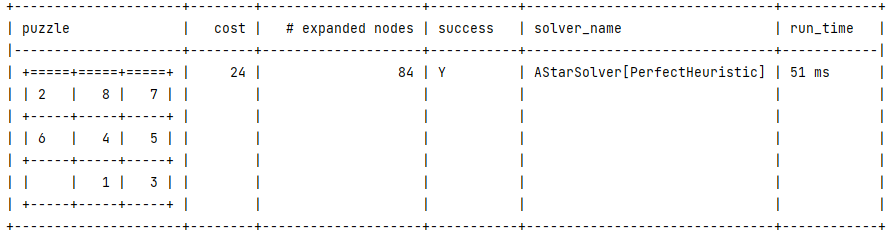
\includegraphics[scale=0.5]{./Figures/exampleastarperfectsolver}
%\decoRule
\caption[Examples]{a* perfect solver example}
\label{fig:exampleastarperfectsolver}
\end{figure}



\Subsubsection{Deep Learning Heuristic}
\Subsubsection{Deep Reinforcement Learning Heuristic}
\Subsubsection{Deep Q Learning Heuristic}


